%
% A (non-exhaustive) list of TODOs:
%


\chapter{PhoG: Photon Gun}\label{chapter:phog}
Goal of chapter: analyse and model the PhoG device and its efficacy for producing, from a classical input, (i) bright sub-Poissonian state; (ii) entangled state


\section{Introduction}
\begin{itemize}
\item Introduce dissipation as a means for state engineering
\item Introduce our goal to produce single-photons (or close to single-photons)
\item Introduce this chapter, include a chapter outline, and provide motivation for why we will look at different models
\end{itemize}

\begin{figure}[htp]
\centering
\includegraphics[draft=false, width=\linewidth]{phog/phog_models}
\caption{\label{fig:phog_models} Hierarchy of models of the phog device, from least realistic (left) to most realistic (right). We will discuss each model in turn throughout the rest of this chapter. \MakeUppercase{\romannumeral 1}: Single-mode model. \MakeUppercase{\romannumeral 2}: Two-mode model. \MakeUppercase{\romannumeral 3}: Three-mode model. \MakeUppercase{\romannumeral 4}: Multi-mode model. \MakeUppercase{\romannumeral 5} Multi-mode model embedded in glass. }
\end{figure}

\section{Single-mode model}

\begin{figure}[htp]
\centering
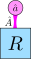
\includegraphics[width=0.2\linewidth, draft=false]{phog/single_mode}
\caption{\label{fig:phog_single_mode} A single bosonic mode, $a$, is coupled to a Markovian reservoir $R$ by operator $\hat{A}$. }
\end{figure}

\MT{Make sure that my analysis in this section is sufficiently motivated and doesn't seem like too much of a detour.}

Consider the model displayed in Fig.~\ref{fig:phog_single_mode} (c.f. Fig.~\ref{fig:phog_models}\MakeUppercase{\romannumeral 1}), which consists of a single bosonic mode, $a$, coupled to a reservoir $R$ via a reservoir operator $\mathcal{A}$. The annihilation (creation) operator for mode $a$ is denoted $\hat{a} \left(\hat{a}^\dagger\right)$, and the density matrix containing all information about the state of the mode is denoted $\rho_a$. This model will prove illustrative of several principles which we will develop throughout the chapter. Assuming that reservoir $R$ is Markovian, the evolution of mode $a$ is given by the following quantum master equation in Lindblad form\footnote{Equations in this form will be referred to as ``Lindblad equations''}

\begin{equation}\label{eqn:phog_lindblad_1}
\ddt \rho_a =  - i \left[\hat{H}, \rho_a\right] + \gamma \mathcal{L}\left(\hat{A}\right)\rho_a
\end{equation}

\noindent In what follows we consider the case with Hamiltonian $\hat{H} = \hbar \omega \hat{a}^\dagger \hat{a}$. Eq.~\ref{eqn:phog_lindblad_1} then describes the decay of state $\rho_a\left(t=0\right)$ into $R$ with rate $\gamma$. The Lindbladian term $\mathcal{L}\left(\hat{A}\right)$ takes the usual form
\begin{equation}\label{eqn:phog_lindbladian_form}
\mathcal{L}\left(\hat{A}\right)\rho_a = \hat{A}\rho_a\hat{A}^\dagger - \frac{1}{2} \hat{A}^\dagger \hat{A} \rho_a - \frac{1}{2} \rho_a \hat{A}^\dagger \hat{A}.
\end{equation}

\noindent Let us consider the behaviour of an initially coherent state $\rho_a\left(t=0\right) = \dyad{\alpha}$ with amplitude $\alpha$. We will explore several choices for decay operator $\hat{A}$.

\subsection{$\hat{A} = \hat{a}$}
First, we will explore the case where the decay into the reservoir is governed by mode $a$ annihilation operator, $\hat{a}$, which corresponds to single-photon loss.% I can refer to intro chapter for properties of this.
The evolution of $\rho_a$ is described by

\begin{equation}\label{eqn:phog_lindblad_single_photon_loss}
\ddt \rho_a = \gamma\left[\hat{a}\rho_a \hat{a}^\dagger - \frac{1}{2} \hat{a}^\dagger \hat{a} \rho_a - \frac{1}{2} \rho_a \hat{a}^\dagger \hat{a}\right],
\end{equation}
where we have transformed into a rotating frame and so the free Hamiltonian term $\hbar \omega \hat{a}^\dagger \hat{a}$ vanishes. Let us calculate the evolution $\langle \hat{a}^\dagger \hat{a}\rangle\left(t\right)$ of photon number expectation:

\begin{align}
\ddt \langle \hat{a}^\dagger \hat{a}\rangle &= \gamma \left[ \text{Tr}\left(\hat{a}^\dagger \hat{a} \hat{a} \rho_a \hat{a}^\dagger \right) - \frac{1}{2} \text{Tr}\left(\hat{a}^\dagger \hat{a} \hat{a}^\dagger \hat{a} \rho_a\right) - \frac{1}{2} \text{Tr}\left(\hat{a}^\dagger \hat{a} \rho_a \hat{a}^\dagger \hat{a}\right)\right] \notag \\
%
&= \gamma \left[ \langle \hat{a}^\dagger \hat{a}^\dagger \hat{a}\hat{a}\rangle - \langle \hat{a}^\dagger \hat{a} \hat{a}^\dagger \hat{a}\rangle \right] \notag \\
%
&= - \gamma \langle \hat{a}^\dagger \hat{a}\rangle
\end{align}
\noindent and so
\begin{equation}\label{eqn:phog_single_photon_loss_number_expectation}
\langle\hat{a}^\dagger \hat{a} \rangle \left(t\right) = \langle \hat{a}^\dagger \hat{a}\rangle \left(0\right) e^{- \gamma t}
\end{equation}
the photon number exponentially decays in time with decay rate $\gamma$. We may derive similar equations for $\langle\hat{x}\rangle\left(t\right)$ and $\langle\hat{x}\rangle\left(t\right)$ and find 
\begin{align}\label{eqn:phog_single_photon_loss_quadrature_expectation}
 \langle \hat{x}\rangle\left(t\right) &= \langle \hat{x}\rangle\left(0\right) e^{- \frac{\gamma}{2} t} \notag \\
%
 \langle \hat{p}\rangle\left(t\right) &= \langle \hat{p}\rangle \left(0\right) e^{- \frac{\gamma}{2} t}.
\end{align}

\noindent We might guess that the steady-state of Eq.~\ref{eqn:phog_lindblad_single_photon_loss} is the vacuum $\dyad{0}$, and indeed we can deduce that this must be the case by noticing that $\ddt \rho_a = 0$ when $\rho_a$ is vacuum. In Fig.~\ref{fig:phog_lindblad_single_photon_loss}a we plot the evolution of $\langle\hat{a}^\dagger \hat{a}\rangle, \langle \hat{x}\rangle, \langle \hat{p}\rangle$ and see that the photon number expectation and quadrature expectations decay towards zero, confirming Eqs.~\ref{eqn:phog_single_photon_loss_number_expectation},~\ref{eqn:phog_single_photon_loss_quadrature_expectation}, while the variances in $\hat{x}$ and $\hat{p}$ remain constant. This might lead us to conclude that the state $\rho_a\left(t\right)$ remains a coherent state with decreasing amplitude $\alpha\rightarrow0$, until it reaches the vacuum state.

In Fig.~\ref{fig:phog_lindblad_single_photon_loss}b we plot the fidelities $\mathcal{F}$ between $\rho_a\left(t\right)$ and the vacuum state $\dyad{0}$, the single-photon state $\dyad{1}$ and a coherent state $\dyad{\alpha^\prime}$ with $\left|\alpha^\prime\right|^2 = \langle \hat{n}\rangle_{\rho_a}\left(t\right)$, in other words the coherent state with same photon-number expectation as $\rho_a$. We observe that the fidelity to the vacuum state increases to $1$ while the fidelity to coherent state $\dyad{\alpha^\prime}=1$ always, which confirms our intuitions that $\rho_a$ remains coherent $\forall t$ and that $\dyad{0}$ is the steady state.


\begin{figure}[htp]
\centering
	\begin{subfigure}{0.6\linewidth}
	\centering
	\includegraphics[draft=false, width=\linewidth]{phog/expects_a}
	\caption{}
	\end{subfigure}
	\begin{subfigure}{0.6\linewidth}
	\centering
	\includegraphics[draft=false, width=\linewidth]{phog/fidelities_a}
	\caption{}
	\end{subfigure}
\caption{\label{fig:phog_lindblad_single_photon_loss}$\hat{A} = \hat{a}$. (a) Operator expectation values calculated for state $\rho_a\left(t\right)$ as it evolves under Eq.~\ref{eqn:phog_lindblad_single_photon_loss}. An initial coherent state $\alpha=3.0$ decays to vacuum state $\dyad{0}$. Quadrature variances remain constant through time, implying that $\rho_a$ remains a coherent state throughout its evolution. This is confirmed in (b) where the fidelity between $\rho_a$ and $\dyad{\alpha^\prime}$ is demonstrated to remain $1$ for all time. The amplitude $\alpha^\prime$ is chosen to give a coherent state with equivalent photon-number expectation to $\rho_a\left(t\right)$. Horizontal gridlines displayed in black, dashed.}
\end{figure}

\subsection{$\hat{A} = \hat{a}^2$}
Next we consider a two-photon loss term $\hat{a}^2$, which describes two-photon decay into the reservoir. Our Lindblad equation is

\begin{equation}\label{eqn:phog_lindblad_two_photon_loss}
\ddt \rho_a = \gamma\left[\hat{a}^2 \rho_a \hat{a}^{\dagger 2} - \frac{1}{2} \hat{a}^{\dagger 2} \hat{a}^2 \rho_a - \frac{1}{2} \rho \hat{a}^{\dagger 2} \hat{a}^2\right]
\end{equation}
which gives the evolution of photon number expectation as 
\begin{equation}
\ddt \langle \hat{a}^\dagger \hat{a}\rangle = - 2 \gamma \langle \hat{a}^\dagger \hat{a}^\dagger \hat{a}\hat{a}\rangle
\end{equation}
which does not take a closed form and so we cannot yet directly calculate $\langle \hat{a}^\dagger \hat{a}\rangle\left(t\right)$. Similarly, equations for evolution of $\langle\hat{a}\rangle\left(t\right)$ require terms to the third power in the creation/annihilation operators, and so are not yet closed.  We will see techniques in Sec.~\ref{sec:linearization} which allow us to deal with this.

\MT{TODO: expand this discussion to allow for mixedness in output state.}
For now, let us deduce what must be the steady-state of Eq.~\ref{eqn:phog_lindblad_two_photon_loss}. We observe that once again the vacuum $\dyad{0}$ must be a steady state, since then $\ddt \rho_a=0$. Surprisingly we now also have the single-photon state $\dyad{1}$ as a steady state since this also has $\ddt \rho_a=0$. The general steady-state is a superposition of these
\begin{equation}\label{eqn:phog_phase_state}
\ket{\psi} = \ket{0} + e^{i \phi} \ket{1} \qq{with} \rho_a\left(t \rightarrow \infty\right) = \dyad{\psi}
\end{equation}
which takes the form of a so-called \emph{phase state}, and has long been known that the steady state of two-photon loss is a phase-state. The phase $\phi$ is related to the phase of the initial coherent state. %\MT{show this.}


In Fig.~\ref{fig:phog_lindblad_two_photon_loss}a we plot the evolution of $\langle \hat{a}^\dagger \hat{a}\rangle, \langle \hat{x}\rangle, \langle \hat{p}\rangle$ and the quadrature variances. The photon number expectation no longer decays to zero as it did for $\hat{A}=\hat{a}$. In Fig.~\ref{fig:phog_lindblad_two_photon_loss}b we observe the fidelity between $\rho_a\left(t\right)$ and the final phase state increases to $\MT{X}$, and so we see that two-photon loss induces nonclassicality in the system. \MT{I should talk about the mixedness of the state somewhere.}


\begin{figure}[htp]
\centering
	\begin{subfigure}{0.6\linewidth}
	\centering
	\includegraphics[draft=false, width=\linewidth]{phog/expects_aa}
	\caption{}
	\end{subfigure}
	\begin{subfigure}{0.6\linewidth}
	\centering
	\includegraphics[draft=false, width=\linewidth]{phog/fidelities_aa}
	\caption{}
	\end{subfigure}
\caption{\label{fig:phog_lindblad_two_photon_loss}$\hat{A} = \hat{a}^2$. (a) Operator expectation values for state $\rho_a\left(t\right)$ as it evolves under Eq.~\ref{eqn:phog_lindblad_two_photon_loss}. An intially coherent state with $\alpha=3.0$ no longer decays to the vacuum state, and the final photon-number expectation is nonzero. The quadrature variances are no longer constant which implies that the state is no longer coherent, which is confirmed in (b) where the fidelity between $\rho_a\left(t\right)$ and $\dyad{\alpha^\prime}$ is plotted. The fidelity between $\rho_a\left(t\right)$ and steady state increases to \MT{X}. Horizontal gridlines displayed in black, dashed.}
\end{figure}



\subsection{$\hat{A} = \hat{a}^3$}
We might guess that the steady state $\ket{\psi}$ of the three-photon loss term $\hat{a}^3$ is likewise a superposition of $\ket{0}, \ket{1}$ and $\ket{2}$
\begin{equation}\label{eqn:phog_three_photon_loss_ss}
\rho_a\left(t\rightarrow\infty\right) = \frac{\dyad{\psi}}{3} \qq{with} \ket{\psi} \stackrel{?}{=} \ket{0} + e^{i \phi}\ket{1} + e^{i \varphi}\ket{2}
\end{equation}
\MT{check how the state is normalized}
with phases $\phi, \varphi$ in general depending on the initial coherent state $\dyad{\alpha}$. %\MT{TODO: investigate this numerically}.
Indeed, we can deduce that Eq.~\ref{eqn:phog_three_photon_loss_ss} must be a steady state of the system by noting that $\hat{a}^3 \ket{\psi} = 0$ which implies $\ddt \rho_a = 0$.

%\MT{TODO: analytically show in fock basis the steady state}

We plot the evolution of fidelities between $\rho_a\left(t\right)$ evolving with decay operator $\hat{a}^3$ in Fig.~\ref{fig:phog_lindblad_three_photon_loss}. We see the fidelity to the state in Eq.~\ref{eqn:phog_three_photon_loss_ss} increasing to \MT{X}. \MT{additional comments.}

\begin{figure}[htp]
\centering
\includegraphics[draft=false, width=0.6\linewidth]{phog/fidelities_aaa}
\caption{\label{fig:phog_lindblad_three_photon_loss}$\hat{A} = \hat{a}^3$ (a) Fidelities between state $\rho_a\left(t\right)$ and vacuum (red), single-photon state (orange), coherent state with equivalent photon-number expectation to $\rho_a$ (green), and the two-phase state (blue). \MT{additional comments/interpretation.} Horizontal gridlines displayed in black, dashed.}
\end{figure}

\clearpage
\subsection{$\hat{A} = \hat{a}\left(\hat{a}^\dagger \hat{a} - 1\right)$}
We have seen that the choice of $\hat{A}$ can give drastically different steady states of $\rho_a$,  from the uninteresting vacuum to the highly quantum and useful phase-state. We therefore wish to consider which choices for $\hat{A}$ will give rise to a Fock state $\dyad{n}$

The choice 
\begin{equation}\label{eqn:phog_A_ncl}
\hat{A} = \hat{a}\left(\hat{a}^\dagger \hat{a} - 1\right)
\end{equation}
may be interpreted as a single-photon loss with a rate which depends on photon number. We can see that the loss rate will go to zero for state $\dyad{1}$, and so suspect that the single-photon state $\dyad{1}$ is a steady state of this loss mechanism.

%The vacuum state $\dyad{0}$ also happens to be a steady-state of $\ncl$, but \MT{its coefficient remains constant, so we obtain $\dyad{1}$ in the limit of $\alpha\rightarrow \infty$}


We examine the evolution of $\rho_a$ in Fig.~\ref{fig:phog_A_ncl} and plot the evolution of photon number, $\langle \hat{x}\rangle, \langle \hat{p}\rangle$ in (a). We observe non-exponential decay of photon-number expectation to $1$ %TODO: show that it is non-exponential. (e.g. try fitting an exponential to it)
while in (b) the fidelity between $\rho_a\left(t\right)$ and $\dyad{1}$ increases to $1$, implying that this choise of $\hat{A}$ does indeed have a single-photon steady state. Even after short times $t < 0.1$ the fidelity to an equivalent coherent state quickly decreases (and the quadrature variances quickly increase over similar timescale), implying a rapid increase in non-classicality of the system.\footnote{We shall explore and quantify this later.}

Therefore, we deduce that the decay operator $\hat{a}\left(\hat{a}^\dagger \hat{a} - 1\right)$ is a useful candidate for driving our system towards the highly nonclassical single-photon state. In the remainder of this chapter our goal will be to find a physical system which can efficiently implement this decay operator.


\begin{figure}[htp]
\centering
	\begin{subfigure}{0.6\linewidth}
	\centering
	\includegraphics[width=\linewidth, draft=false]{phog/expects_ncl1}
	\caption{}
	\end{subfigure}
	\begin{subfigure}{0.6\linewidth}
	\centering
	\includegraphics[width=\linewidth, draft=false]{phog/fidelities_ncl1}
	\caption{}
	\end{subfigure}
\caption{\label{fig:phog_A_ncl}$\hat{A} = \hat{a}\left(\hat{a}^\dagger \hat{a} - 1\right)$ (a) Operator expectation values for state $\rho_a\left(t\right)$ as it evolves. An initially coherent state with $\alpha=3.0$ decays to a state with $\langle \hat{n}\rangle=1$, which we confirm as state $\dyad{1}$ by considering the fidelity in (b). Horizontal gridlines displayed in black, dashed.}
\end{figure}

Before we move on, let us quickly explore the related operator $\hat{a}\left(\hat{a}^\dagger \hat{a} -2\right)$. Based on the above discussion we might reasonably expect the steady-state to be $\dyad{2}$, and this is indeed what we see in Fig.~\ref{fig:phog_A_ncl2}, where the fidelity to the two-photon state increases to $1$.

\begin{figure}[htp]
\centering
\includegraphics[width=0.6\linewidth, draft=false]{phog/fidelities_ncl2}
\caption{\label{fig:phog_A_ncl2}}
\end{figure}



\clearpage
\section{Including loss}
We have seen that the loss operator $\ncl$ is a good canditate for driving an initial coherent state towards a single photon state $\ket{1}$. Any system, therefore, which can implement the Lindblad equation~\ref{eqn:phog_lindblad_1} with $\hat{A} = \ncl$ will asymptotically give rise to single-photon Fock states. 

